% Combined author-selected sampling panels; main figure numbering is preserved.
\clearpage
\newcounter{samplingfigurebackup}
\setcounter{samplingfigurebackup}{\value{figure}}
\begingroup
\renewcommand{\thefigure}{B\arabic{figure}}
\ifdefined\theHfigure\renewcommand{\theHfigure}{budgetoption.\arabic{figure}}\fi
\setcounter{figure}{0}
\section*{Combined sampling figure}
This figure presents Qwen, LoQI, FlowR, and NExT-Mol using the same fixed-target
ensembles as Table~\ref{tab:recovery} and the initial Qwen checkpoint.
For each entry, let $N$ be the number of candidates presented to PoseBusters,
$h(t)$ the number of retained conformers within RMSD threshold $t$, and
$k=\min(K,N)$ for requested budget $K$. A uniform subset without replacement
recovers the entry with probability
\[
 p(K,t)=1-\frac{\binom{N-h(t)}{k}}{\binom{N}{k}}.
\]
Rejected candidates remain non-hits. We average these probabilities over all
94 entries. This evaluates sampling within the saved pools, rather than raw
generation attempts or computational cost. Uncertainty in panel A
uses the same bootstrap entry weights across methods, thresholds, and budgets.

\begin{figure}[p]
\centering
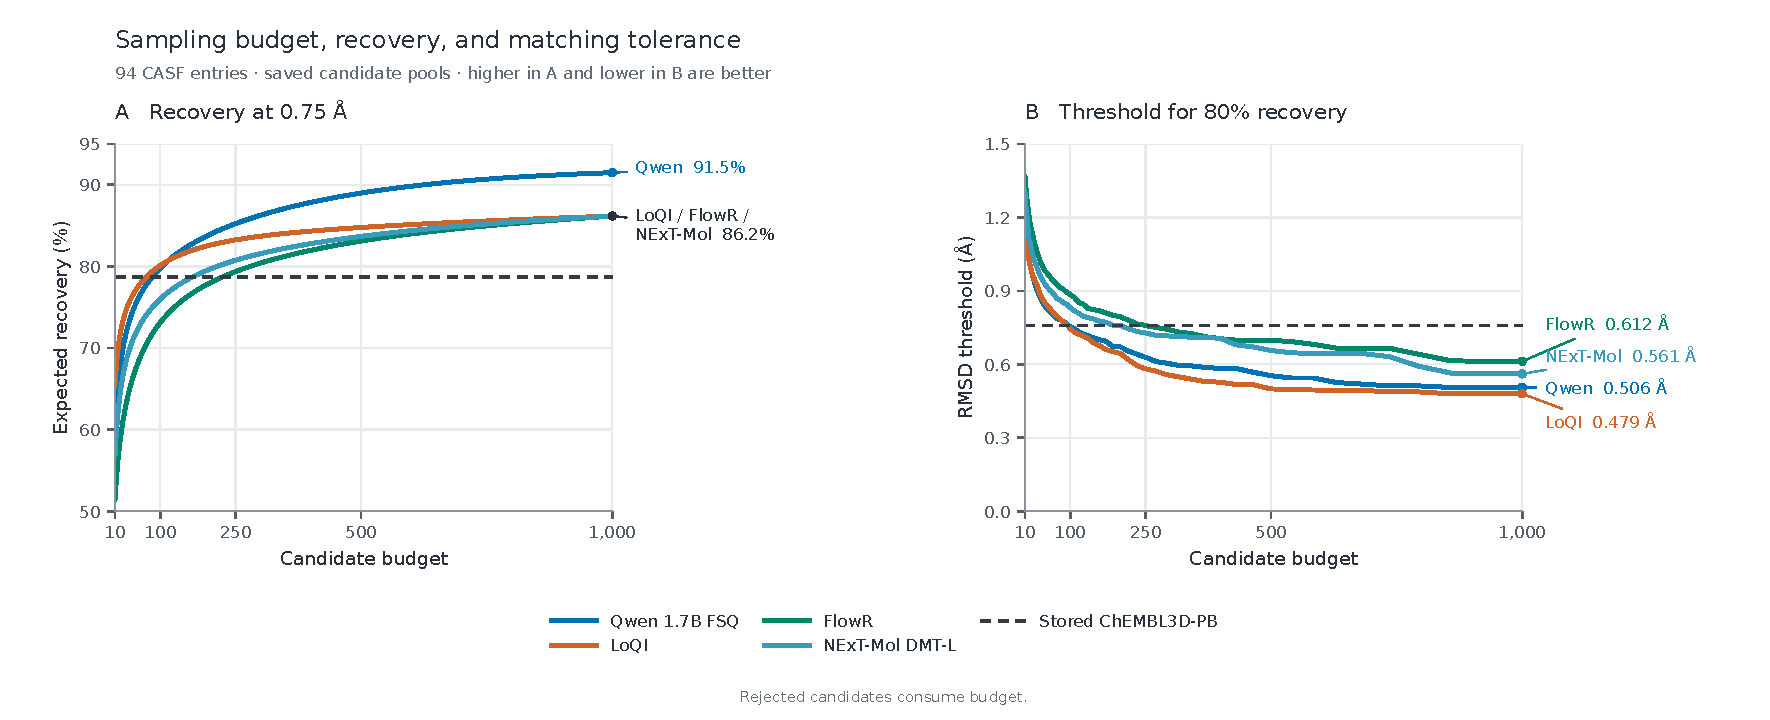
\includegraphics[width=\linewidth]{figures/figure-budget-combined.pdf}
\caption{Sampling performance of Qwen, LoQI, FlowR, and NExT-Mol. (A) Expected recovery at RMSD $\leq$ 0.75 \AA{} as a function of candidate budget; higher is better. Shading gives pointwise 95\% percentile intervals from 2,000 paired entry-bootstrap resamples. (B) Smallest RMSD threshold required for 80\% expected recovery at each budget; lower is better. The threshold varies in panel B, while the recovery target is fixed. Both panels use exact recovery probabilities for uniform subsets drawn without replacement from the saved pre-PoseBusters candidate pools, averaged over all 94 CASF entries. Rejected candidates consume budget, empty retained ensembles count as failures, and budgets are capped at the available candidate count. Dashed lines show the full stored ChEMBL3D-PB ensemble at the corresponding criterion. Intervals in A are conditional on the saved pools; panel B is descriptive without uncertainty bands. The 80\% target is a presentation choice, and neither panel extrapolates beyond 1,000 candidates.}
\label{fig:sampling-option-b1}
\end{figure}
\clearpage
\endgroup
\setcounter{figure}{\value{samplingfigurebackup}}
